\section{Introduction}

\begin{figure}[h]
\begin{center}
%\fbox{\rule{0pt}{2in} \rule{1.0\linewidth}{0pt}}
   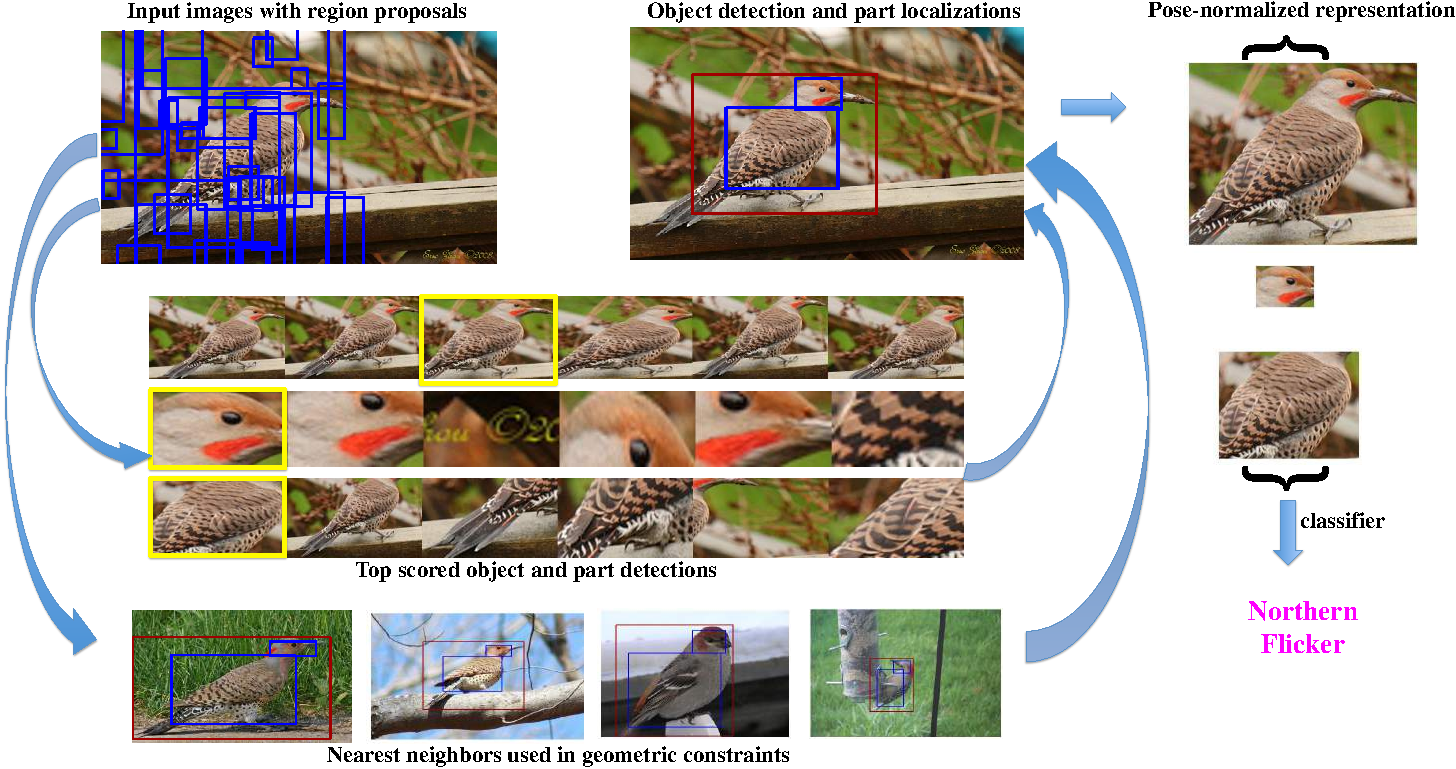
\includegraphics[width=0.99\linewidth]{concept.pdf}
\end{center}
   \caption{\textbf{Overview of our part localization}  Starting from bottom-up region proposals (top-left), we train both object and part detectors based on deep convolutional features. During test time, all the windows are scored by all detectors (middle), and we apply non-parametric geometric constraints (bottom) to rescore the windows and choose the best object and part detections (top-right).  The final step is to extract features on the localized semantic parts for fine-grained recognition for a pose-normalized representation and then train a classifier for the final categorization. Best viewed in color.} 
\label{fig:concept}
\end{figure}

   
The problem of visual fine-grained categorization can be extremely challenging due to the subtle differences in the appearance of certain parts across related categories. In contrast to basic-level recognition, fine-grained categorization aims to distinguish between different breeds or species or product models, and often requires distinctions that must be conditioned on the object pose for reliable identification. Facial recognition is the classic case of fine-grained recognition, and it is noteworthy that the best facial recognition methods jointly discover facial landmarks and extract features from those locations. 

Localizing the parts in an object is therefore central to establishing correspondence between object instances and discounting object pose variations and camera view position. Previous work has investigated part-based approaches to this problem~\cite{poof,BirdletsFarrellICCV11,iccv13_keypoint,UW_NIPS12,PosePoolingKernelsZhangEtalCVPR12,Goering14:NPT}. The bottleneck for many pose-normalized representations
% , including that proposed by Farrell et al.,
is indeed accurate part localization.
The Poselet \cite{BourdevMalikICCV09} and DPM \cite{dpm} methods have previously been utilized to obtain part localizations with a modest degree of success; methods generally report adequate part localization only when given a known bounding box at test time~\cite{Tricos_Chai_ECCV12,iccv13_alignment,ParkhiEtalICCV11,ParkhiEtalCVPR12,iccv13_partmatching}. By developing a novel deep part detection scheme, we propose an end-to-end fine grained categorization system which requires no knowledge of object bounding box at test time, and can achieve performance rivaling previously reported methods requiring the ground truth bounding box at test time to filter false positive detections.

The recent success of convolutional networks, like~\cite{krizhevsky}, on the ImageNet Challenge~\cite{ILSVRC} has inspired further work on applying deep convolutional features to related image classification~\cite{decaf} and detection tasks~\cite{rcnn}.
In~\cite{rcnn}, Girshick et al. achieved breakthrough performance on object detection by applying the CNN of~\cite{krizhevsky} to a set of bottom-up candidate region proposals~\cite{selsearch}, boosting PASCAL detection performance by over 30\% compared to the previous best methods.
Independently, OverFeat~\cite{overfeat} proposed localization using a CNN to regress to object locations.
However, the progress of leveraging deep convolutional features is not limited to basic-level object detection.
In many applications such as fine-grained recognition, attribute recognition, pose estimation, and others, reasonable predictions demand accurate part localization.

Feature learning has been used for fine-grained recognition and attribute estimation, but was limited to engineered features for localization.
DPD-DeCAF~\cite{dpd} used DeCAF~\cite{decaf} as a feature descriptor, but relied on HOG-based DPM~\cite{dpm} for part localization.
PANDA~\cite{panda} learned part-specific deep convolutional networks whose location was conditioned on HOG-based poselet models.
These models lack the strength and detection robustness of R-CNN~\cite{rcnn}.
In this work we explore a unified method that uses the same deep convolutional representation for detection as well as part description.

We conjecture that progress made on bottom-up region proposal methods, like selective search~\cite{selsearch}, could benefit localization of smaller parts in addition to whole objects.
As we show later, average recall of parts using selective search proposals is 95\% on the Caltech-UCSD bird dataset.

In this paper, we propose a part localization model which overcomes the limitations of previous fine-grained recognition systems by leveraging deep convolutional features computed on bottom-up region proposals.
Our method learns part appearance models and enforces geometric constraints between parts.
An overview of our method is shown in Figure~\ref{fig:concept}. We have investigated different geometric constraints, including a non-parametric model of joint part locations conditioned on nearest neighbors in semantic appearance space.
We present state-of-the-art results evaluating our approach on the widely used fine-grained benchmark Caltech-UCSD bird dataset~\cite{DatasetCUB200}.

% \todo{
% an important distinction of us vs PANDA, DPD-kdes, and DPD-KNN (and poselets-attributes) is that we have a clean story with single deep network archicture for all parts of our system: detection, part localization, part description}
% 
% just answer the question: on average, are the parts easier or harder to detect than the whole?
%and/or how much do we lose with selective search?
%
%can the r-cnn method also detect parts"?
%"is selective search salient for parts"?
%
%does the decaf feature reveal parts?"
